%!TEX root = main.tex
\paragraph{Uncontrolled dynamics}
	We split the the constant population $N$ in a base SEIR
structure with segregation infected classes according with
manifestation  of symptoms. We also postulate the extra state $Y_{I_S}$ to fit commulative symptomatic cases reported in the databases from Mexico city
during the exponential grow phase. Our dynamics reads
\begin{equation}
	\label{eqn:base_dynamics}
    \begin{aligned}
    	L' & = \theta \mu N^{\star}
        	-\epsilon \lambda L - \delta_L L - \mu L,
    	\\
    	S' & =
        	(1 - \theta)\mu N^\star + \delta_L  L + \delta_R R
        	- (\lambda + \mu) S,
    	\\
    	E' & =
        	\lambda (\epsilon L + S) - (\kappa + \mu) E,
    	\\
    	I_S' & =
        	p \kappa E -
        	(\gamma_S +
        	    \delta_H +
        	    \deleted[id=SDIV]{\mu_{I_S}} +
        	    \mu) I_S,
    	\\
    	I_A' &=
        	(1 - p) \kappa E - (\gamma_A + \mu) I_A,
    	\\
    	H' &=
        	\delta_H I_S - (\gamma_H + \mu_H + \mu) H,
    	\\
    	R' & =
        	\gamma_S I_S + \gamma_A I_A + \gamma_H H - (\delta_R + \mu) R,
    	\\
    	D' &=
        	\deleted[id=SDIV]{\mu_{I_S} I_S +} \mu_H H,
    	\\
    	\frac{dY_{I_S}}{dt} &  = p \kappa E,
    	\\
    	\lambda &:=
        	\frac{\beta_A I_A + \beta_S I_S}{N^{\star}},
    	\\
    	N^{\star}(t) &=
        	L + S + E +
       	 	I_S + I_A +
        	H + R .
    \end{aligned}
\end{equation}
%
     See \Cref{tbl:dynamics_base_parameters} for notation and references
     values.
\begin{table*}[h!]
	\centering
	\begin{tabular}{>{\centering}%
        p{0.2\textwidth}%
        p{0.4\textwidth}
    }
		\toprule
		\textbf{Parameter} & \textbf{Description}
  	\\
  	\midrule
		$\mu$ &
			Death rate
		\\
        $\beta_S$ &
        	Infection rate between susceptible and symptomatic infected
		\\
        $\beta_A$ &
        	Infection rate between susceptible and asymptomatic infected
		\\
        $\lambda_V$ &
        	Vaccination rate
		\\
        $\delta_{V}^{-1}$ &
        Vaccine-induced immunity
		\\
        $\varepsilon$ &
        	Vaccine efficacy
		\\
        $\kappa^{-1}$ &
        	Average incubation time
        \\
		$p$ &
			New asymptomatic generation proportion
		\\
	    $\theta$ &
        	Proportion of individuals under lockdown
        \\
        $\gamma_{S}^{-1}$ &
        	Average time of symptomatic recovery
        \\
		$\gamma_{A}^{-1}$ &
			Recovery average time of asymptomatic individuals
		\\
		$\gamma_{H}^{-1}$ &
			Recovery average time by hospitalization
		\\
        $\delta_{R}^{-1}$ &
        	Natural immunity
  		\\
  		$\delta_{H}$ &
        	Infected symptomatic hospitalization rate
  		\\
  	\bottomrule
	\end{tabular}
		\caption{
			Parameters definition of model in
			\Cref{eqn:base_dynamics}.}
    \label{tbl:dynamics_base_parameters}
\end{table*}
%
\begin{figure*}[htb]
    \centering
    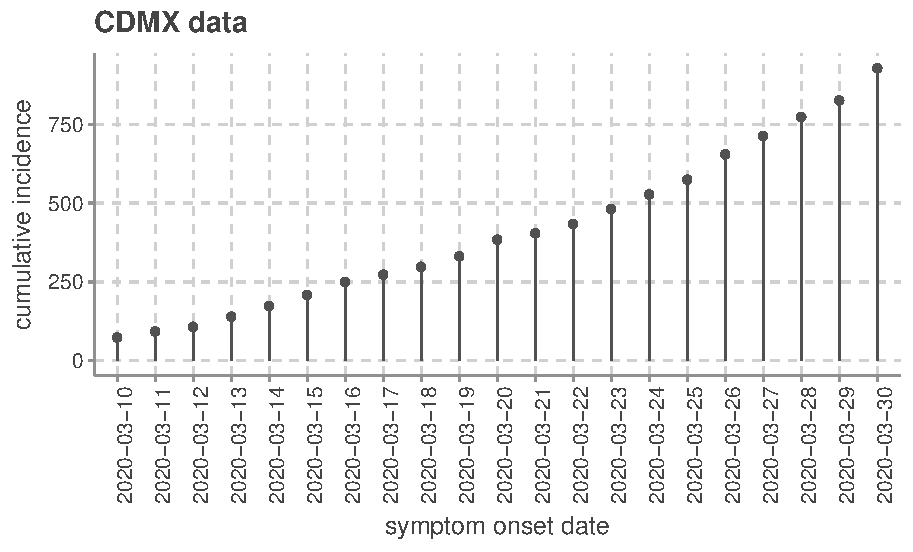
\includegraphics[scale=0.8, keepaspectratio]{./cdmx_input_data}
    \caption{%
        Cummulative new symptomatic and confirmed COVID19 reported cases from
        Ciudad de Mexico between March, 10, to March 30 of 2020.
    }
    \label{fig:data_CDMX}
\end{figure*}
%
\begin{figure*}[htb]
	\centering
   	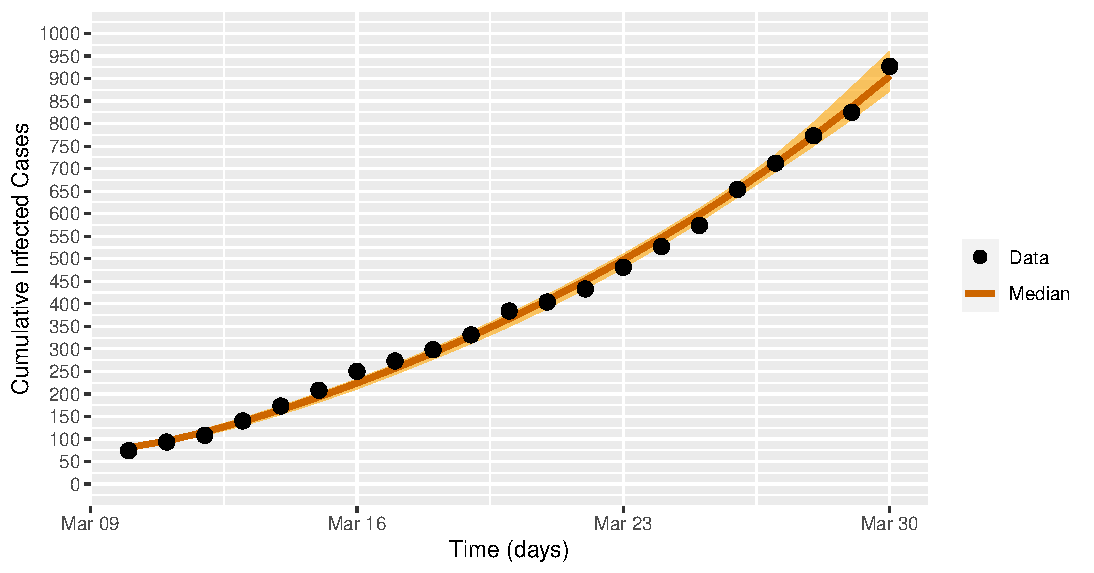
\includegraphics[scale=0.8, keepaspectratio]{./cdmx_CIs_data_begining_fit}
   	\caption{%
   		Fit of diary new cases of Mexico city
   		during exponential growth.
   	}
    \label{fig:data_CDMX_fitting}
\end{figure*}
%
    \paragraph{Hypothesis} 
    	We consider that susceptible individuals become
    infected when they are in contact with asymptomatic individuals and
    individuals with symptoms, we will propose that a proportion of
    asymptomatic individuals have a way to get relief and not die. A
    proportion of individuals infected with symptoms may die from the
    disease or may be relieved.

    	We callibrate parameters of our base dynamics in
    \eqref{eqn:base_dynamics} via Multichain Montecarlo (MCMC).
    To this end, we assume that the comulative
    incidence of new infected symptomatic cases $CI_S$
    follows a Poisson distribution with mean $\lambda_t = IC_s(t)$. Further,
    following [] we postulate priors for $p$ and $\kappa$
    \begin{equation}
    	\label{eqn:boservation_model}
    	\begin{aligned}
    		Y_t & \sim Poisson(\lambda_t),
    		\\
    		\lambda_t
    			&=
    			\int_{0}^t p \delta_e E ,
    		\\
    			& p \sim \text{Uniform} (0.3, 0.8),
    		\\
    			& \kappa \sim \text{Gamma}(10, 50).
    	\end{aligned}
    \end{equation}
	
	Using the reproductive number definition of VanDenDrishe, we obtain
\begin{equation*}
	\label{eqn:reproductive_number}
	R_0 :=
		\frac{
			N^{*}(
				\beta_S p
				\kappa +
				\beta_A
				\kappa(1-p) )
		}{
			(\mu - \kappa)( \gamma_S + \mu_{I_s} + \gamma_A + \mu)
			N^* \mu
		}
\end{equation*}

    \Cref{fig:data_CDMX_fitting} displays data of coumulative confirmed cases 
of COVID-19 of Mexico city, and the fitt of our model in
\Cref{eqn:base_dynamics,eqn:boservation_model}.
